%%%%%%%% ICML 2019 EXAMPLE LATEX SUBMISSION FILE %%%%%%%%%%%%%%%%%

\documentclass{article}

% Recommended, but optional, packages for figures and better typesetting:
\usepackage{microtype}
\usepackage{graphicx}
\usepackage{subfigure}
\usepackage{amsmath}
\usepackage{booktabs} % for professional tables
\usepackage[latin1]{inputenc}
\usepackage{tikz}

\usetikzlibrary{shapes,arrows}

% Define block styles

\tikzstyle{block} = [rectangle, draw, fill=blue!20, 
text width=5em, text centered, rounded corners, minimum height=2em, node distance=2cm]
\tikzstyle{block8} = [rectangle, draw, fill=blue!7, 
text width=5em, text centered, rounded corners, minimum height=2em, node distance=2cm, minimum width=8cm]
\tikzstyle{block10} = [rectangle, draw, fill=blue!7, 
text width=5em, text centered, rounded corners, minimum height=2em, node distance=2cm, minimum width=10cm]
\tikzstyle{bigblock10} = [rectangle, draw, fill=red!20, 
text width=5em, text centered, rounded corners, minimum height=4em, minimum width=10cm]
\tikzstyle{bigblock14} = [rectangle, draw, fill=red!20, 
text width=5em, text centered, rounded corners, minimum height=4em, minimum width=14cm]
\tikzstyle{line} = [draw, -latex']


% hyperref makes hyperlinks in the resulting PDF.
% If your build breaks (sometimes temporarily if a hyperlink spans a page)
% please comment out the following usepackage line and replace
% \usepackage{icml2019} with \usepackage[nohyperref]{icml2019} above.
\usepackage{hyperref}

% Attempt to make hyperref and algorithmic work together better:
\newcommand{\theHalgorithm}{\arabic{algorithm}}

% Use the following line for the initial blind version submitted for review:
\usepackage[accepted]{icml2019}
% \usepackage[style=authoryear]{biblatex}
% \addbibresource{example_paper.bib}
% If accepted, instead use the following line for the camera-ready submission:
%\usepackage[accepted]{icml2019}

% The \icmltitle you define below is probably too long as a header.
% Therefore, a short form for the running title is supplied here:
\icmltitlerunning{Submission and Formatting Instructions for ICML 2019}

\begin{document}

\twocolumn[
\icmltitle{Extending BERT for multi-choice problems \\}

% It is OKAY to include author information, even for blind
% submissions: the style file will automatically remove it for you
% unless you've provided the [accepted] option to the icml2019
% package.

% List of affiliations: The first argument should be a (short)
% identifier you will use later to specify author affiliations
% Academic affiliations should list Department, University, City, Region, Country
% Industry affiliations should list Company, City, Region, Country

% You can specify symbols, otherwise they are numbered in order.
% Ideally, you should not use this facility. Affiliations will be numbered
% in order of appearance and this is the preferred way.
\icmlsetsymbol{equal}{*}

\begin{icmlauthorlist}
\icmlauthor{Orr Dermer}{equal,cs}
\icmlauthor{Afek Adler}{equal,in}
\end{icmlauthorlist}

\icmlaffiliation{in}{Department of Industrial Engineering, University of Tel Aviv, Tel Aviv, Israel}
\icmlaffiliation{cs}{Department of Computer Science, University of Tel Aviv, Tel Aviv, Israel.}


\icmlcorrespondingauthor{Afek Adler}{afekilayadler@gmail.com}
\icmlcorrespondingauthor{Orr Dermer}{odermer@gmail.com}

% You may provide any keywords that you
% find helpful for describing your paper; these are used to populate
% the "keywords" metadata in the PDF but will not be shown in the document
\icmlkeywords{Machine Learning, NLP}

\vskip 0.3in
]

% this must go after the closing bracket ] following \twocolumn[ ...

% This command actually creates the footnote in the first column
% listing the affiliations and the copyright notice.
% The command takes one argument, which is text to display at the start of the footnote.
% The \icmlEqualContribution command is standard text for equal contribution.
% Remove it (just {}) if you do not need this facility.

%\printAffiliationsAndNotice{}  % leave blank if no need to mention equal contribution
\printAffiliationsAndNotice{\icmlEqualContribution} % otherwise use the standard text.

\begin{abstract}
Deep learning models are still far away from human-level performance in commonsense reasoning tasks.
We introduce a multi-choice question answering scheme that models the dependencies between answers by
building a relationship graph between the answers for a given question. 
then, we compute a centrality measure for each node (answer) in the graph and predict the answer by taking the node with the maximum value of that centrality measure.
We test ourselves on the challenging CommonsenseQA dataset and show that although our method is capable of modeling more complex relationships between the answers we did not manage to improve the current state of the art on this task.
\end{abstract}

\section{Introduction}
When we face a multi-choice question answering (QA) problem where we have to choose the most 
probable answer we arrive at it with prior information and knowledge. for instance, we have some kind of a

Whereas in some cases the state of the art machine-learning methods which were trained on massive amount of data to infer prediction roles
outperforms human-level by a large margin (e.g. SQUAD 2.0 \cite{rajpurkar2018know}),
In the field of common sense reasoning  \cite{talmor2018commonsenseqa} state of the art algorithms fail to generalize and are yet inferior to human level performance.
this is due to two main reasons. first, is that when using algorithms such as fine-tuning a pre-trained language model, it is likely that this knowledge (common sense) does not exist explicitly in the pre training corpus. and second, is due to the fact that creating massive datasets for this purpose solely is hard, and developed only in the last years mostly by crowdsourcing.

Due to this inherent difficulty of this methods the research community invests resources in creating larger-scale datasets in different difficulty levels, e.g., the SWAG \cite{zellers2018swag} dataset with ~100K examples where \cite{devlin2018bert} demonstrate a model which is already at a human level and the CommonseneQA \cite{talmor2018commonsenseqa} a dataset which was made especially for common sense reasoning with \~{}10K samples where the state of the art is much lower then human-level. for a detailed survey of resources see \cite{storks2019commonsense}. 

In this work, we suggest and evaluate models which eliminate the Independence assumption between answers for a given question, aiming to improve the benchmark on the CommonsenseQA dataset. 

\section{Background and Related Work}
Research on machine common sense QA has long been acknowledged for it's critical component in natural language understanding. but only recently with the embracing of deep learning in natural language processing and crowdsourcing to create larger scale datasets, major breakthroughs has emerged; to the best of the author's knowledge, the first large scale common sense reasoning QA dataset was introduced is 2018 \cite{storks2019commonsense}.

Due to the fact that the prominent approach to to solve common sense QA problems is with word embeddings (WE) and contextualized word embeddings (CWE) in the next section we will provide a brief introduction to CVE and explain how to use it in the context of common sense QA.

% We would like to note that this paper address specifically solutions for multi-choice QA with common sense reasoning and not closely related themes such as visual commonsense reasoning or co reference resolution.

\subsection{Contextualized Word Embeddings}
Based on the pioneering work of Word2Vec \cite{mikolov2013distributed} which enabled words to be represented as vectors, those
enriching the information contained in the input for a variation of language based machine learning tasks, many models extended the Word2Vec concept by taking context into account; the same word has a different meaning in different context. the leading approaches to obtain a contextualized word representations is using the hidden layer of an LSTM \cite{hochreiter1997long} and more specifically a biLSTM such as in ELMO \cite{peters2018deep} or more recently using a transformer architecture such as \cite{devlin2018bert,yang2019xlnet}.

The great power of WE or CWE is to enable using a generic method as a basis for task specific machine learning models; for instance, in natural language processing there are many different tasks (e.g. machine translation, sentiment analysis) and a simple model based on CWE with fine tuning on a given dataset usually provides much better results than previous models on a given task, creating a new bencmark for this specific task. the fact that mega companies provides those trained models as an open source service makes it easy to use for academics and in the industry as one.

CWE is a type of transfer learning method; a model is pretrained on a base dataset and fine tuned on the task dataset,  with the underlying hypothesis that information distilation is possible from one source (base dataset) to the other (task specific dataset).
The main reason for the great success of CWE is that the base model is trained using supervised learning on huge amounts of data, e.g. BERT, was trained on 3.3B words. the fact that CWE models are also self trained makes it easier to collect such huge amount of data without the need to label examples. the downside of this models is that they use many parameters (BERT Large - 340M) - so trainig and infering requires large processing power and latency is a challenge for creating real time systems. in the next section we will introduce the benchmark model which we aim to improve - BERT for CommonsenseQA (which is identical to BERT for SWAG) as was introduced in the original paper of BERT.

\subsection{BERT}
BERT is a word based CWE model that was pre-trained on two learning objectives. given a sentence, predict masked words (15\% of the words were masked) and next sentence prediction. BERT’s  model  architecture is a multi-layer bidirectional Transformer encoder \cite{vaswani2017attention} with the following hyper-parameters (BERT Large) - 12 Transformer blocks, hidden size 1024 (H) and 16 self attention heads. BERT input can be one or two sentences.

BERT input representation (figure \ref{bert_input_repr}) uses WordPeace \cite{wu2016google} tokenization which is a data driven method that aims to achieve a balance between vocabulary size and out-of-vocab words. this way BERT stores only 30K vocabulary words very rarely encounter out-of-vocab words when tokenizing English texts. two special token are added for each sentence, a start token [CLS] and an end token [SEP]. if the input contains two sentences another [CLS] token is added in between the sentences. Due to the fact that Transformers do not encode the sequential nature of their inputs a segment ids and position embeddings are added as well to the input.

\begin{figure}[ht]
\vskip 0.2in
\begin{center}
\centerline{\includegraphics[width=\columnwidth]{bert_input_repr}}
\caption{input representation for BERT (from the original paper).}
\label{bert_input_repr}
\end{center}
\vskip -0.2in
\end{figure}
fine tuning BERT is simply swapping out the appropriate input and output, whether the input is a single text or a text pair the input and output pairs are given to the model and the parameters are fine-tuned by back-propagation end to end after connecting to the [CLS] token embedding to a task specific classification layer with a given loss function. 

\subsection{BERT baseline for SWAG}

In the BERT Paper, the authors approach the SWAG challange with the following input (figure \ref{fig:model_orig}). that input is fed to BERT architecture and the [CLS] token embedding is used to predict a logit by calculating a dot product with a learned vector. this process is done for each answer independently of each other and then a softmax layer with cross entropy loss is calculated to compute the error. As we can see, this architecture introduce only H (1024) new parameters to the existing BERT model.


% \begin{equation}
% [CLS][Question][SEP][Answer][SEP] 
% \label{original_input_order}
% \end{equation} 

\section{CommonSeneseQA}
CommonSeneseQA is a dataset which specifically made for common sense reasoning, by asking crowd workers to generate questions from concepts from ConceptNet. it contains 12,247 examples and 5 answers per question. 
the Authors use the same architecture as in the BERT benchmark for SWAG
and report Accuracy score of 56.7\%. The current state of the art
on this dataset is currently 68.3\% accuracy, 23.6\% below human level.

\section{Methodology}
We propose a method with different variants to model the dependencies between answers, by feeding answer pairs jointly to BERT's architecture. by doing so, we contribute by:
\begin{itemize}
\item making the model more expressive by removing the independence assumption
\item extending the model to deal with questions as 'what is largest?"
\item  extending the model to deal with answers as 'all answer are correct" or 'none of the above"
\end{itemize}

\section{Methodology}

We derive our model from the BERT baseline for SWAG. However, as we want our model to compare between the different possible answers, we deviate from the original model by introducing the model with the question and 2 possible answers as each input sequence, for which the model returns a score - 1 meaning the first answer is more likely, and 0 if the second answer is the likeliest. Having received a score for each of pairs, we then integrate those into probability scores for each of the original answers - and then choose the one with the highest probability as our predicted answer.

\subsection{Dataset alterations}

In the original paper, each input sequence consisted of a classifier token ('[CLS]'), the question, a separator token ('[SEP]'), a possible answer, and then another separator token, as seen in figure \ref{fig:model_orig}. The classifier token is unique, as the final hidden state corresponding to that token was used as the aggregate sequence representation for the question-answering task.

\tikzset{
	font={\fontsize{12pt}{12}\selectfont}}

\begin{figure}[h!]
\begin{center}
\scalebox{0.7}{
	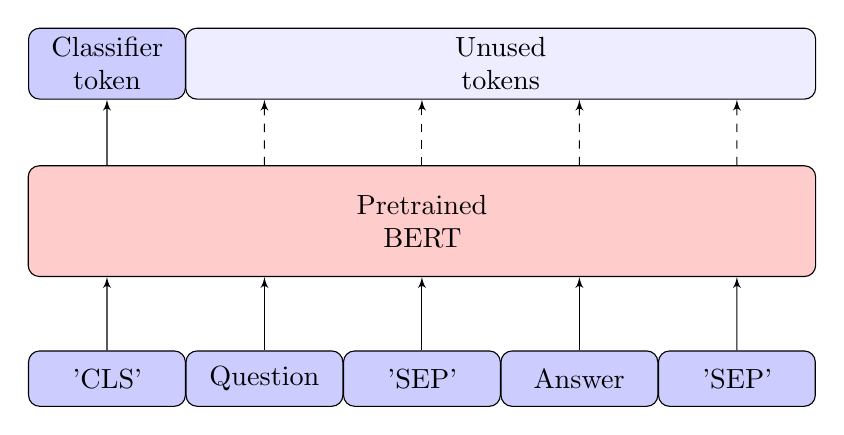
\begin{tikzpicture}[node distance = 2cm, auto]
	\node [bigblock10] (bert) at (0,0) {Pretrained BERT };
	\node [block, below of=bert] (SEP1) {'SEP'};
	\node [block, left of=SEP1] (question) {Question};
	\node [block, left of=question] (CLS) {'CLS'};
	\node [block, right of=SEP1] (answer) {Answer};
	\node [block, right of=answer] (SEP2) {'SEP'};
	\node [block] (classifier) at (-4,2) {Classifier token};
	\node [block8] (rest) at (1,2) {Unused tokens};
	\path [line] (CLS) -- ([xshift=-4cm]bert.south);
	\path [line] (question) -- ([xshift=-2cm]bert.south);
	\path [line] (SEP1) -- (bert.south);
	\path [line] (answer) -- ([xshift=2cm]bert.south);
	\path [line] (SEP2) -- ([xshift=4cm]bert.south);
	\path [line] ([xshift=-4cm]bert.north) -- (classifier.south);
	
	\path [line,dashed] ([xshift=-2cm]bert.north) -- ([xshift=-3cm]rest.south);
	\path [line,dashed] ([xshift=-0cm]bert.north) -- ([xshift=-1cm]rest.south);
	\path [line,dashed] ([xshift=2cm]bert.north) -- ([xshift=1cm]rest.south);
	\path [line,dashed] ([xshift=4cm]bert.north) -- ([xshift=3cm]rest.south);
	
	\end{tikzpicture}
}
\end{center}
\caption{The original paper's question-answering model.}
\label{fig:model_orig}
\end{figure}

Our model deviates from these assumptions. Instead, each input sequence was constructed from the question and 2 possible answers in the following manner: A classifier token, the first answer, a separator token, the question, a separator token, the second answer, and another classifier token (As seen in figure \ref{fig:model}). Note, that this construction break several of the original BERT paper assumptions - each of our input sequences consist of more than just one classifier token, and more than just two sentences. As such, it is possible that BERT will suffer from reduced performance, as its entire training process was built around these assumptions.
However, breaking these assumptions was a crucial part of what made our constructions work - it allowed for each of the classifier tokens to "absorb" the meaning of the answer closer to it, and imporved the symmetry of our model in regard to each of the two answers.


\tikzset{
	font={\fontsize{13pt}{14}\selectfont}}

\begin{figure}[h!]
\begin{center}
	\scalebox{0.6}{
		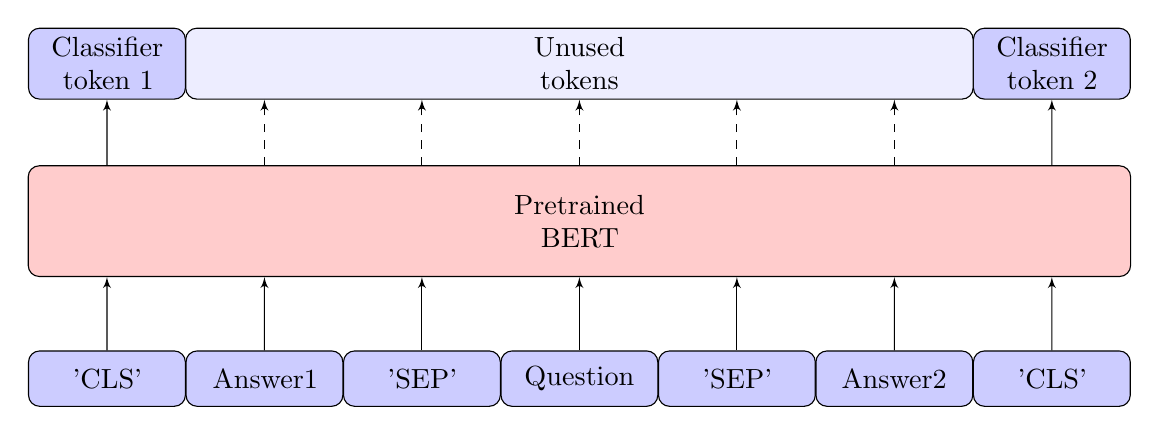
\begin{tikzpicture}[node distance = 2cm, auto]
		\node [bigblock14] (bert) at (0,0) {Pretrained BERT};
		\node [block, below of=bert] (Question) {Question};
		\node [block, left of=Question] (Sep1) {'SEP'};
		\node [block, left of=Sep1] (Answer1) {Answer1};
		\node [block, left of=Answer1] (Cls1) {'CLS'};
		\node [block, right of=Question] (Sep2) {'SEP'};
		\node [block, right of=Sep2] (Answer2) {Answer2};
		\node [block, right of=Answer2] (Cls2) {'CLS'};
		\node [block] (classifier1) at (-6,2) {Classifier token 1};
		\node [block] (classifier2) at (6,2) {Classifier token 2};
		\node [block10] (rest) at (0,2) {Unused tokens};
		
		\path [line] (Cls1) -- ([xshift=-6cm]bert.south);
		\path [line] (Answer1) -- ([xshift=-4cm]bert.south);
		\path [line] (Sep1) -- ([xshift=-2cm]bert.south);
		\path [line] (Question) -- (bert.south);
		\path [line] (Sep2) -- ([xshift=2cm]bert.south);
		\path [line] (Answer2) -- ([xshift=4cm]bert.south);
		\path [line] (Cls2) -- ([xshift=6cm]bert.south);
		
		
		\path [line] ([xshift=-6cm]bert.north) -- (classifier1.south);
		\path [line] ([xshift=6cm]bert.north) -- (classifier2.south);
		
		\path [line,dashed] ([xshift=-4cm]bert.north) -- ([xshift=-4cm]rest.south);
		\path [line,dashed] ([xshift=-2cm]bert.north) -- ([xshift=-2cm]rest.south);
		\path [line,dashed] ([xshift=-0cm]bert.north) -- ([xshift=-0cm]rest.south);
		\path [line,dashed] ([xshift=2cm]bert.north) -- ([xshift=2cm]rest.south);
		\path [line,dashed] ([xshift=4cm]bert.north) -- ([xshift=4cm]rest.south);
		\end{tikzpicture}
	}
\end{center}
\caption{Our question-answering model.}
\label{fig:model}
\end{figure}

% $$
% P := \text{\textit{Learned parameter}}
% $$
% $$
% CT_{i,j} := \text{\textit{Classifier Tokens Concatened}}
% $$
% $$
% S'_{i,j} := P \cdot CT_{i,j}
% $$
% $$
% \text{\textit{Score}}_{i,j} := \frac{S'_{i,j} + (1 - S'_{j,i})}{2}
% $$

Another part of the input sequence given to BERT is the segment embeddings - a number from \{0, 1\} which signifies whether the current token is part of the first sentence or the second. After trial and error, it was found that we perform best when giving a value of 1 for \textbf{each} of the answer tokens, and 0 for the question tokens. That makes sense, as part of the desire for symmetry in our model, and the fact that BERT wasn't trained with a possibility for a third sentence, so using, for example, the number 2 for our second answer would not make any sense to it.

After passing our input sequence through BERT, we use a concatenation of the final hidden states matching the classifier tokens as the sequence representation. We learn as a parameter a vector whose dot product with the sequence representation is the score for the given answer pair (equation \ref{edge_score}). than, we compute the edge score between answers i to j by 'averaging' the sigmoid result of the two. add a sentence \# \ \# \# \# \# \#


\begin{equation}
  \label{eq:t}
  \begin{aligned}
      \vec{CT_{i,j}} &:= \text{\textit{Classifier Tokens Concatenated}}\\ 
    \vec{P} &:= \text{\textit{Learned parameters}}\\
    S'_{i,j} &:= sigmoid(\vec{CT_{i,j}} \cdot \vec{P})\\
    \text{\textit{Score}}_{i,j} &:= \frac{S'_{i,j} + (1-S'_{j,i}))}{2}
  \end{aligned}
  \label{edge_score}
\end{equation}

\subsection{Pair scores integration}

We conceived a few methods of combining the different pair scores into probabilities for the answers. In this section we will review those methods and compare them.

\subsubsection{Learnt weights}

In this method, we introduce more layers to derive the indiviual probabilities from the pair scores. We used 2 layers, with a hidden size of $ (number\ of\ pairs)^2 $ and normalizing with a softmax layer.

\subsubsection{Markov chains}

In this method, we find the stationary distribution of a weighted graph whose edge's weights are derived from our pair scores.
The reasoning for this process is as follows - imagine a graph whose vertices are the given answers. We begin by choosing an answer randomly, and we want to move on to the best possible answer. At each time step, we move to a different answer, choosing based on the scores of the pairs in which our current answer participates, i.e. the better another answer performed against our current answer, the more likely we are to move to it.
This process is powerful, because it captures the dependency between the different answers, e.g. if answer B is better than answer A, and answer C is better than answer B,\# \# \# \# \#
than we'd like to factor in that information when comparing between answers A and C. 

% TODO: add a markov chain graph here

Simply constructing a matrix with each cell being the score for the matching pair, normalizing each row so that we have a probability matrix, and then calculating the stationary distribution doesn't work well in practice. This is because normalizing the matrix causes the model to be unable to capture the absolute value of the scores, e.g. if it sees a row in which all values are similar, it can't differ the case in which all scores were low (and thus our "current" answer is good) from the case all of the scores were high.
Consider the following matrix:

$$
\begin{bmatrix}
0 & 0.95 & 0.85 & 0.25 \\
0.05 & 0 & 0.98 & 0.74 \\
0.15 & 0.02 & 0 & 0.45 \\
0.75 & 0.26 & 0.55 & 0
\end{bmatrix}
$$

We can see that the third answer had won in every comparison - thus, we would expect it to be assigned the highest probability. Given the currently described method, this in not the case, as the probabilities received would be:
$$ \begin{bmatrix} 0.22614831 & 0.16630443 & 0.29576885 & \textbf{0.31177841} \end{bmatrix} $$

We solve this problem by adding the average of each column to the matching cell on the diagonal. This makes sense, as this gives us the option of staying on the current choice, and the better a certain choice had performed against the other choices, the greater the possibility of staying on it.
After doing this, we derive this matrix for our example:

$$
\begin{bmatrix}
\textbf{0.31} & 0.95 & 0.85 & 0.25 \\
0.05 & \textbf{0.41} & 0.98 & 0.74 \\
0.15 & 0.02 & \textbf{0.79} & 0.45 \\
0.75 & 0.26 & 0.55 & \textbf{0.48}
\end{bmatrix}
$$

And this probability matrix for our choices:
$$ \begin{bmatrix} 0.16845236 & 0.13252954 & \textbf{0.43521662} & 0.26380148 \end{bmatrix} $$

\subsubsection{Tie-breakers}

This is not a method on its own, but it can be used on top of the other ones.
Essentially, we can assert a "Certainty Threshold" on the probabilities obtained from the other methods, a rate between two probabilities under which we consider our prediction to be uncertain/unstable.
If such a scenario arises, we then resort to choosing between the two highest-scored choices directly - that is, by looking at the score given to the pair and deciding accordingly.

Note that this change does not cause a change in the probabilities themselves, it only changes the predicted answer. As such, it does not cause a change in the measured loss, thus does not affect the learned parameters. It does change, however, the measured accuracy, which means that when learning parameters we will favor a parameter set that maximizes the accuracy given this change.

\section{Experiments and Results} 

As our model deviates greatly from the assumptions that were made when the original BERT weights were trained, it is understandable that our model required more epochs to converge than the amount of epochs the original paper used when fine-tuning to the question answering task.
We should also note that because each sample now consists of much more input sequences (the original model had one sequence per possible answer, our model has one sequence per possible answer \textbf{pair}), we are now more limited in our batch size, as the GPU has to hold the entire batch simultaneously. This problem can be mitigated by using gradient accumulation.

Our models were trained in parts.
In the first part, we trained solely on the dataset alterations part, without integrating the pair scores. That is, our model was trained directly on identifying the better answer from a pair of answers. After 5 epochs with a dynamic learning rate (starting from 1e-6 and decreasing to 4e-7) we were able to achieve a 70.3\% accuracy on the dev set. (Note that this accuracy is measured over pairs and not over questions - it is not comparable to the performance of other models over this dataset).

In the second part, we trained our model for 2 more epochs using each method of pair-scores integration suggested. Empirically, using the tie-breakers method on any of the suggested models caused a drop in performance, and thus it was discarded.
A comparison of our experiment results follows.

\begin{table}[h!]
	\label{tbl:accuracy}
	\vskip 0.15in
	\begin{center}
		\begin{small}
			\begin{sc}
				\begin{tabular}{lr}
					\toprule
					Method	& Accuracy (dev-set)\\
					\midrule
					Comparative Model + \\ \qquad \qquad Markov chains 	& 49.3\% \\
					Comparative Model + \\ \qquad \qquad Learnt weights 	& 49.1\% \\
					\midrule
					Random guess & 25\% \\
					Original BERT model (baseline) & \textbf{56.7\%} \\
					\bottomrule
				\end{tabular}
			\end{sc}
		\end{small}
	\end{center}
	\vskip -0.1in
	\caption{Full model comparison}
\end{table}

\section{Discussion}
\subsection{Train-Test Discrepancy}
when humans tackle multi-choice questions we compare all answer pairs simultaneously, disqualify some unreasonable answers and approve others before we make a prediction. those, we narrow the number of possible solutions in a multi-phase process. in this paper, this is exactly what we wanted to achieve when we compared all answers pairs altogether. we believe that our model under performed because of Train Test Discrepancy; we are aiming to learn in a supervised way information which is not exactly given to us - in the training set, we know only the gold labels per each question and not the relationship between them. therefore, there is no information about answers which are totally wrong or answers which are close to each other and can be the prediction candidates. 

as well, in the training phase we create 4 answer pairs - the gold answer with all the other answers (number of answers - 1) and at test time we create all possible answer pairs which is 20. it appears that at training time the model learns to discriminate between the right answer and the wrong answer. a dynamic which is not necessarily the same at test time when we feed all answer pairs together. this discrepancy can be inherent in the dataset and the way it was built. e.g , it may be that the gold answer is better then all the other candidate answer but some answers are distractors which ``confuse" the model at test time.

\subsection{Conclusions}
Neither the Markovian model nor the Learnt weights model outperformed the baseline model, in fact there was a siginficant gap between our methods and the baseline results. we believe that it is due to a combination of the following reasons:
\begin{itemize}
\item train-test discrepancy issue.
\item BERT was trained in a different manner than our architecture. it is likely  that our input representation has harmed the information distillation from the original BERT model those harming the final result. it is still an open question which input configuration is optimal in the sense that information from BERT model is kept but also answer pair information is learned. 
\item  bigger datasets can help in this manner in order to be able to generalize well input configurations that is different then BERT baseline. as well, bigger datasets  can allow more freedom to use larger models with more parameters. in the current model we have 5 samples per each parameter learned which requires large regularization, possibly more complex generalization rules.
\end{itemize}

\section{Future Work}
To solve the train-test discrepancy issue, we believe that it is possible to create a dataset with more detailed training labels, for example, ranking the answers and providing information about distractor answers. it is interesting to verify if we can achieve a better performance by removing this discrepancy.

Another interesting idea to do with a ranked dataset is to fully ``neuralize"" our Markov chain solution. one way to do that can be by feeding all the answer pairs jointly to  BERT, compute a logit to every pair and compare it with the ranked ground troth ,than use a graph convolutional layers to classify the correct answer. it can also be interesting to examine the graph layer of this network for explainability reasons.  

% In the unusual situation where you want a paper to appear in the
% references without citing it in the main text, use \nocite
\nocite{langley00}

\bibliography{example_paper}
\bibliographystyle{icml2019}


%%%%%%%%%%%%%%%%%%%%%%%%%%%%%%%%%%%%%%%%%%%%%%%%%%%%%%%%%%%%%%%%%%%%%%%%%%%%%%%
%%%%%%%%%%%%%%%%%%%%%%%%%%%%%%%%%%%%%%%%%%%%%%%%%%%%%%%%%%%%%%%%%%%%%%%%%%%%%%%
% DELETE THIS PART. DO NOT PLACE CONTENT AFTER THE REFERENCES!
%%%%%%%%%%%%%%%%%%%%%%%%%%%%%%%%%%%%%%%%%%%%%%%%%%%%%%%%%%%%%%%%%%%%%%%%%%%%%%%
%%%%%%%%%%%%%%%%%%%%%%%%%%%%%%%%%%%%%%%%%%%%%%%%%%%%%%%%%%%%%%%%%%%%%%%%%%%%%%%
%%%%%%%%%%%%%%%%%%%%%%%%%%%%%%%%%%%%%%%%%%%%%%%%%%%%%%%%%%%%%%%%%%%%%%%%%%%%%%%
%%%%%%%%%%%%%%%%%%%%%%%%%%%%%%%%%%%%%%%%%%%%%%%%%%%%%%%%%%%%%%%%%%%%%%%%%%%%%%%

% \printbibliography
\end{document}


% This document was modified from the file originally made available by
% Pat Langley and Andrea Danyluk for ICML-2K. This version was created
% by Iain Murray in 2018, and modified by Alexandre Bouchard in
% 2019. Previous contributors include Dan Roy, Lise Getoor and Tobias
% Scheffer, which was slightly modified from the 2010 version by
% Thorsten Joachims & Johannes Fuernkranz, slightly modified from the
% 2009 version by Kiri Wagstaff and Sam Roweis's 2008 version, which is
% slightly modified from Prasad Tadepalli's 2007 version which is a
% lightly changed version of the previous year's version by Andrew
% Moore, which was in turn edited from those of Kristian Kersting and
% Codrina Lauth. Alex Smola contributed to the algorithmic style files.
